\documentclass[aps,prl,twocolumn,superscriptaddress,amsmath,amssymb,floatfix]{revtex4-2}
\usepackage{graphicx}
\usepackage{xcolor}
\usepackage{bm}
\usepackage[colorlinks=true,allcolors=blue]{hyperref}
\renewcommand{\topfraction}{0.95}
\renewcommand{\bottomfraction}{0.95}
\renewcommand{\textfraction}{0.05}
\renewcommand{\floatpagefraction}{0.85}

\begin{document}

\title{Classes of metamaterials generated by recursive cell division}

\author{Alexei Vazquez}
\email{alexei@nodeslinks.com}
\affiliation{Nodes \& Links Ltd, Salisbury House, Station Road, Cambridge, CB1 2LA, UK}

\date{\today}

\begin{abstract}
The physical properties of metamaterials depend on a balance between their fine structure and
their long-range features. Periodic lattices are stiff because straight lines of struts span
them. Quasicrystals are ordered without being periodic. Scale-rich metamaterials are
disordered and bend under load. We ask what classes of materials exist given the interplay
between structural order and the alignment of struts into straight spanning lines. We generate
material designs by recursive cell division. We cut each cell at a fraction $r_0$ of its length
from one of its two ends. The value of $r_0$ sets the order class, but the rule that chooses
the end determines the alignment class, and the alignment class determines the elasticity. As a
corollary, the same golden split gives an aligned, stretch-dominated quasicrystal when $r_0$ is
always measured from the same end, and a non-aligned, bending-dominated one when it is measured
from the end that avoids crossings. In that case, for slender frameworks, the
share of the stiffness carried by stretching vanishes as $T^{-1/2}$ with the number of cuts $T$.
\end{abstract}

\maketitle

\begin{figure}[b]
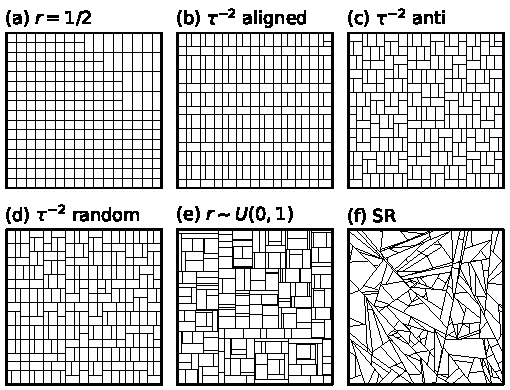
\includegraphics[width=\columnwidth]{fig1.pdf}
\caption{Divisions of the unit square after $T=233$ cuts. (a)--(e) The largest cell is cut
perpendicular to its long side. (a) Periodic grid, $r_0=1/2$. (b)--(d) Golden split
$r_0=\tau^{-2}$, with $r_0$ always on the low side (aligned), on the side that avoids
X-crossings (anti-aligned), and on a random side. (e) Uniform split, $r\sim U(0,1)$. (f)
Scale-rich rule (SR): cell picked by area, cut through a uniform point at a uniform angle.}
\label{fig:div}
\end{figure}

The physical properties of metamaterials depend on a balance between their fine structure and
their long-range features. A periodic lattice of struts is stiff because straight lines of
struts span it and carry load by stretching~\cite{deshpande2001}. A quasicrystal is ordered
without being periodic and diffracts with sharp Bragg peaks~\cite{shechtman1984}. Examples are the
quasicrystalline frameworks built on Penrose and other rhombus tilings, which are Maxwell
lattices whose mechanics follow from the tiling~\cite{stenull2014,zhou2019}. Scale-rich
metamaterials~\cite{both2026} are disordered instead. They are grown by recursive random cell
division, have ligaments of all lengths and few lines that span the sample, and carry load
mainly by bending.

These examples suggest two distinct classifications. One is order, as determined by
diffraction. Order can be periodic, quasiperiodic or disordered (absence of order). The other
is alignment, as determined by whether struts join into straight lines that span the sample.
If the number $m$ of spanning lines grows with the number of cuts $T$ as $m\propto T^{\mu}$,
a framework is aligned for $\mu=1/2$, the largest value when cells have comparable sizes,
non-aligned for $\mu=0$, and partially aligned in between. Alignment fixes how a framework carries load. A framework is
stretch dominated if its stiffness survives when the rigid joints are replaced by pins, and
bending dominated if it does not~\cite{deshpande2001}; spanning lines are what survive. In the
periodic and scale-rich examples order and alignment go together: the periodic lattice is
aligned, the scale-rich metamaterial non-aligned. We ask whether the order class of a
framework fixes its alignment class, and with it the elasticity. Quasiperiodic order is the
critical case. Order requires a rule that repeats itself, repeated cuts line up across
neighbouring cells, and lined-up cuts join into spanning lines, so one may expect quasicrystals
to be aligned and stretch dominated.

Recursive cell division contains the three order classes in one model. It belongs to Cowan's
family of iterated cell divisions~\cite{cowan2010}, defined by which cell is cut, where and at
what angle. Scale-rich metamaterials cut a cell through a random point at a random angle. If
instead each cut lies at a fixed fraction $r_0$ of the cell length, measured from one of the
two sides of the cell, the family contains the periodic grid ($r_0=1/2$) and quasiperiodic
tilings~\cite{baake2013,smilansky2020}. The rule then has two parts, the value of $r_0$ and
the side from which it is measured, and we vary them independently. We treat the order with
the number theory of substitution tilings. We connect alignment to mechanics with an exact
result: for a framework of horizontal and vertical bars with pinned joints, the stiffness
counts the straight lines that span the sample.

\textit{Rules.}---We grow a division of the unit square by $T$ cuts (Fig.~\ref{fig:div}). At
each step the cell of largest area is cut (ties by birth order), perpendicular to its long side
(squares vertically), so all cells stay rectangles. Each cut is a ligament whose two ends lie
on existing ligaments, its hosts, where they form T-junctions. The cut lies at a fraction
$r_0$ of the cell length from one side, so the daughter on that side receives the area
fraction $r_0$ and the other $1-r_0$. The side rule chooses that side, i.e.\ the end of the cell from which $r_0$ is measured:
\emph{aligned}, always the low side (left or bottom);
\emph{random}, a fair coin;
\emph{anti-aligned}, the side that forms fewer X-crossings. An X-crossing is a cut end that
lands on a junction already present on the host from the other side, so that two cuts continue
each other across the host. Ties go to the low side, so the rule is deterministic.
For $r_0=1/2$ both sides coincide; the periodic grid has no anti-aligned version, and the
anti-aligned rule concerns non-periodic order only. As a random reference, the uniform split
$r\sim U(0,1)$ draws a new fraction for every cut; it is the split law induced by the
scale-rich rule~\cite{vazquez2026div}.

With the largest cell cut first and $r_0$ fixed, every cell area has the form
$r_0^{a}(1-r_0)^{b}$, and all cells lie within a fixed size window: the largest is at most
$1/\min(r_0,1-r_0)$ times the smallest, for every side rule. The cells take finitely many
shapes when both fractions are powers of a single number, $r_0=\theta^{-p}$ and
$1-r_0=\theta^{-q}$, with coprime integers $p\ge q\ge1$ and $\theta>1$ a root of
\begin{equation}
x^{p}-x^{p-q}-1=0 .
\label{eq:theta}
\end{equation}
The order then depends on the arithmetic of $\theta$, and in particular on whether $\theta$ is
a Pisot number: an algebraic integer larger than one whose other roots, its Galois conjugates,
all lie inside the unit circle. The golden mean $\tau$ is the best-known example. For $p\le7$
the only rational case is the periodic grid ($p=q=1$, $\theta=2$), and $\theta$ is an
irrational Pisot number for $(p,q)=(2,1)$, $(3,1)$, $(3,2)$, $(4,1)$ and $(5,1)$. These give
$\tau$, $1.466$, the plastic number $\rho$, $1.380$, and again $\rho$, since
$x^{5}-x^{4}-1=(x^{2}-x+1)(x^{3}-x-1)$~\cite{siegel1944}. The five Pisot splits have between
three and six cell shapes up to similarity. The other $(p,q)$ give non-Pisot $\theta$, and an
incommensurate $r_0$, such as $0.3$, gives a number of shapes that grows with
$T$~\cite{smilansky2020}.

\textit{Order.}---Every junction coordinate is a finite sum of powers $\theta^{-k}$ multiplied
by $r_0$ or $1-r_0$, so all coordinates belong to the ring $\mathbb Z[\theta]$. Replacing
$\theta$ by one of its conjugates maps each coordinate to a shadow coordinate. For Pisot
$\theta$ the shadows, measured in units of the smallest cell, stay bounded, because the sum of
powers of a conjugate of modulus below one converges. Together with the size window, this makes
the junction set a Meyer set: its points, and the differences between them, are uniformly
separated, and they fill the plane without large holes. Meyer sets diffract like quasicrystals,
with a relatively dense set of Bragg peaks of positive intensity~\cite{strungaru2005}, as in the Pisot
substitution tilings~\cite{bombieri1986,solomyak1997}. The argument uses only the arithmetic of
the coordinates, not where each cut was placed, so it holds for every side rule. It fails for
non-Pisot $\theta$, whose conjugates are not all inside the unit circle, and when cells are
picked by area, which removes the size window.

\begin{figure*}[t]
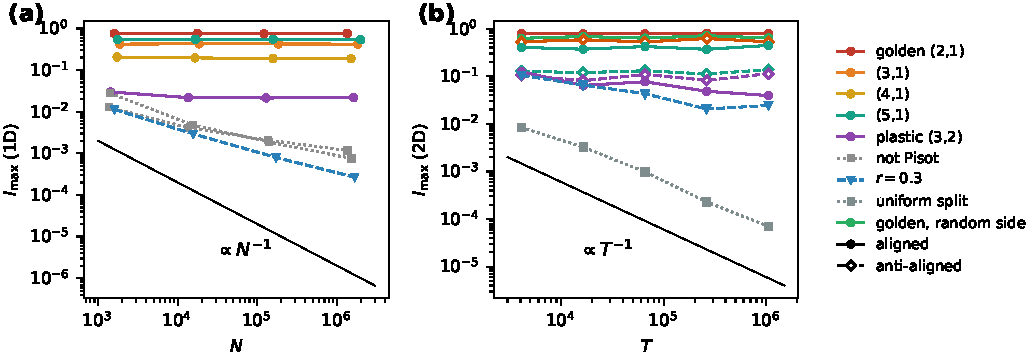
\includegraphics[width=\textwidth]{fig2.pdf}
\caption{Weight of the brightest diffraction peak, $I_{\max}=\max_q S(q)/N$, searched over
$q/2\pi\in[0.25,2]\,N$ (1D) or $[0.25,2]\,T^{1/2}$ (2D, along an axis), around the inverse
mean spacing. A Bragg peak keeps $I_{\max}$ constant; a diffuse spectrum follows the lines
$\propto N^{-1}$ ($T^{-1}$). (a) One-dimensional split sequences with $N$ points, the factors of
the aligned grids. (b) Junction sets of the two-dimensional divisions after $T$ cuts; filled
symbols aligned, open symbols anti-aligned.}
\label{fig:order}
\end{figure*}

We test this through the weight of the brightest peak, $I_{\max}=\max_q S(q)/N$, where
$S(q)=N^{-1}|\sum_j e^{iqx_j}|^{2}$ is the structure factor of $N$ points on a line. A Bragg
peak keeps $I_{\max}$ finite as $N$ grows, whereas a diffuse spectrum gives
$I_{\max}\propto N^{-1}$. In one dimension [Fig.~\ref{fig:order}(a)] every Pisot split keeps a
constant weight over three decades of $N$, while the non-Pisot and incommensurate splits decay
toward the diffuse level. The arithmetic decides whether peaks exist, not how bright they are:
the $(5,1)$ and plastic $(3,2)$ splits share $\theta$, yet their weights differ by a factor
$25$, set by the shape of each substitution's window in shadow space~\cite{baake2013}. In two
dimensions [Fig.~\ref{fig:order}(b)] the brightest peaks lie along the axes. The anti-aligned
weights are lower than the aligned ones but stay constant up to $T=10^{6}$. The side rule
changes the intensities of the Bragg peaks, not their presence.

\textit{Aligned divisions are grids.}---The aligned rule creates straight load paths for a
simple reason: the position of each cut depends only on the extent of the cell across the
cut. A horizontal cut of a cell spanning heights $[y_0,y_0+h]$ lies at $y_0+r_0h$, whatever the
width of the cell, and vertical cuts never change the heights of a cell. Consider the cells of
a horizontal row, which all span the same $[y_0,y_0+h]$. Each of them is eventually cut
horizontally, always at the same height $y_0+r_0h$, so the row splits into two rows along a
line that crosses its whole width. By induction on the rows and, in the same way, on the
columns, the tessellation is a partially refined product $X\times Y$ of two one-dimensional
$r_0$-sequences, each with $(1.1$--$1.3)\,T^{1/2}$ coordinates. Its order is that of its
one-dimensional factors [Fig.~\ref{fig:order}(a)]. Its completed lines span the sample, and
their number $m$ grows as $m\propto T^{\mu}$ with exponent $\mu=1/2$ [Fig.~\ref{fig:mech}(a)];
bounds above and below by multiples of $T^{1/2}$ follow from the size window of the
cells~\cite{supp}. Aligned divisions are therefore in the aligned class whatever their order. The grid requires the same
side in every cell, not the largest-first pick: picking cells by area keeps the spanning
lines.

\textit{Anti-aligned divisions.}---The anti-aligned rule continues a cut across its host only
when both candidate positions would form an X-crossing. Crossings therefore still occur, but at
a minority of the ligament ends, whereas in aligned divisions they occur at nearly all of them.
In our divisions no line other than the first cut ever spans the sample: $m=1$, so $\mu=0$, for all five
Pisot splits up to $T=10^{6}$, and the longest other straight line is the second cut at every
$T$. This is an observation, not a theorem. Anti-aligned divisions are therefore in the
non-aligned class, together with the uniform split and the scale-rich rule. The random side is
partially aligned, with $\mu\approx0.2$.

\textit{Exact pinned stiffness.}---To connect lines with stiffness, we treat the ligaments as
elastic bars of thickness $\lambda$ and Young's modulus $E$, the frame of the square included,
and tile the division periodically. With pinned joints the bars resist only stretching. A
horizontal bar then constrains only the horizontal displacements of its two ends, and a
vertical bar only the vertical ones~\cite{bolker1979}. Under a horizontal strain
$\varepsilon_{xx}$, a horizontal straight line that ends on vertical bars translates rigidly at
no cost, because vertical bars do not resist horizontal motion; only a line that spans the
period must stretch. Each spanning line contributes $E\lambda$, however many bars it is made of,
and shear costs nothing. Per unit area,
\begin{equation}
C^{\rm pin}_{11}=E\lambda\,(m_h+1),\quad C^{\rm pin}_{22}=E\lambda\,(m_v+1),\quad C^{\rm pin}_{66}=0,
\label{eq:Cpin}
\end{equation}
where $m_h$ and $m_v$ count the horizontal and vertical spanning lines and the $1$ is the
frame. Equation~(\ref{eq:Cpin}) agrees to machine precision with finite-element calculations
for aligned, random-side and anti-aligned divisions~\cite{supp}.

The stiffness sets the speed $c$ of long-wavelength sound. We measure it by the index
$n=c_0/c$, where $c_0$ is the sound speed in the solid of the ligaments; a large $n$ means a
slow, compliant material. With the areal density of solid $\bar\rho=\lambda L_{\rm tot}$, where
$L_{\rm tot}\propto T^{1/2}$ is the total ligament length, Eq.~(\ref{eq:Cpin}) gives the
largest possible index along $x$,
\begin{equation}
n_{\max,x}^{2}=\frac{E\bar\rho}{C^{\rm pin}_{11}}=\frac{L_{\rm tot}}{m_h+1}\propto T^{1/2-\mu},
\label{eq:nmax}
\end{equation}
at any density. Rigid joints only add stiffness, so they lower $n$ below this ceiling.
Equation~(\ref{eq:nmax}) ties the elasticity to the alignment class alone. The aligned class,
$\mu=1/2$, has a ceiling that does not grow with $T$. The non-aligned class, $\mu=0$, has a
ceiling that grows as $T^{1/4}$, for anti-aligned quasicrystals and random tessellations alike
[Fig.~\ref{fig:mech}(b)].

\begin{figure*}[t]
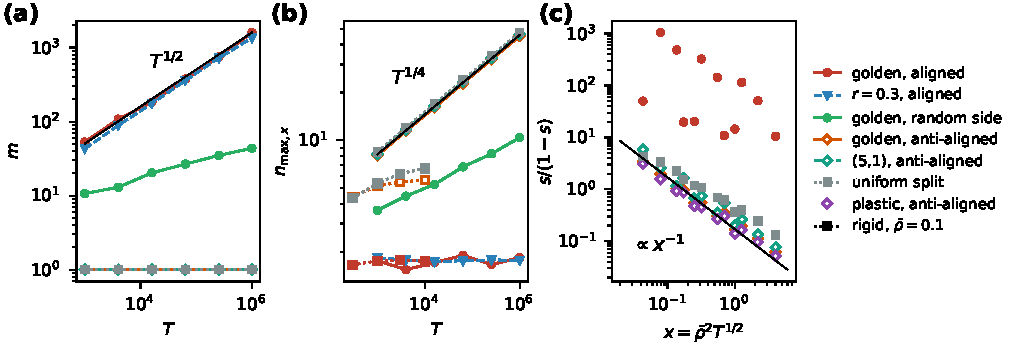
\includegraphics[width=\textwidth]{fig3.pdf}
\caption{(a) Number $m$ of straight lines spanning the square. (b) Index $n=c_0/c$ along $x$:
largest possible value from the pinned stiffness, Eq.~(\ref{eq:nmax}) (lines), and value with
rigid joints at $\bar\rho=0.1$ (squares). (c) Stretching share $s=C^{\rm pin}/C$ of the
rigid-joint stiffness (trace), for $\bar\rho=0.05$, $0.1$, $0.2$ and $T=300$--$10^{4}$; line:
Eq.~(\ref{eq:share}), shown for the anti-aligned splits. Open symbols: anti-aligned.}
\label{fig:mech}
\end{figure*}

\textit{Stretching share.}---Rigid joints add a bending term to the stretching term, $C\simeq
C^{\rm pin}+C^{\rm b}$. The stretching share $s=C^{\rm pin}/C$ is the fraction of the stiffness
that survives when the joints are pinned. It tends to one in a stretch-dominated framework and
to zero in a bending-dominated one~\cite{deshpande2001}. Its dependence on size follows from
scaling. The cells of a fixed-$r_0$ division stay in a fixed size window, so ligament segments
have length $\ell\propto T^{-1/2}$ and thickness $\lambda=\bar\rho/L_{\rm tot}\propto
\bar\rho\,T^{-1/2}$. Their bending gives $C^{\rm b}\propto E(\lambda/\ell)^{3}\propto
E\bar\rho^{3}$, independent of $T$, while Eq.~(\ref{eq:Cpin}) gives $C^{\rm pin}\propto
E\bar\rho\,(m+1)/L_{\rm tot}$. For $m=1$,
\begin{equation}
\frac{s}{1-s}=\frac{C^{\rm pin}}{C^{\rm b}}\propto\frac{1}{\bar\rho^{2}L_{\rm tot}}
\propto\frac{1}{\bar\rho^{2}T^{1/2}} .
\label{eq:share}
\end{equation}
For aligned divisions $m+1\propto L_{\rm tot}$, so $C^{\rm pin}\propto E\bar\rho$ does not vanish
with $T$, and $s$ stays close to one. The excess $C-C^{\rm pin}$ is then not $\propto\bar\rho^{3}$,
because the incomplete parts of the grid lines also carry axial load through the rigid joints,
and Eq.~(\ref{eq:share}) does not apply.

Figure~\ref{fig:mech}(c) tests Eq.~(\ref{eq:share}) with a rigid-joint beam
model~\cite{supp}. Aligned divisions keep $s>0.9$ at every size: their index sits at its
ceiling, and they are stretch dominated. For the three anti-aligned Pisot splits, and for the
random uniform split, the data follow $s/(1-s)\propto x^{-1}$ with $x=\bar\rho^{2}T^{1/2}$
approximately. The dependence on $T$ matches Eq.~(\ref{eq:share}), with fitted exponents
between $-0.5$ and $-0.6$; the dependence on density is weaker, $\bar\rho^{-1.6}$, probably
because of the same axial load in incomplete lines~\cite{supp}. The stretching
share vanishes as the division is refined, and the index grows much more slowly than its
ceiling [Fig.~\ref{fig:mech}(b)]. At $\bar\rho=0.1$ and $T=10^{4}$, stretching carries $14\%$
of the stiffness of the golden anti-aligned division and $94\%$ of the aligned one. The
non-aligned class is therefore bending dominated, whether the division is quasiperiodic or
random.
This conclusion does not rest on the frame of the square: thinning the frame a thousandfold
changes their index by less than $20\%$.

\textit{Finite thickness.}---Real ligaments have a thickness, which limits the result in two
ways. Both limits are densities nearly independent of $T$, because all lengths scale as
$T^{-1/2}$.
First, beam theory needs segments longer than they are thick. The anti-aligned rule moves cuts
away from the cuts on the other side of the host, which creates short host segments. Segments
shorter than three thicknesses stay below $3\%$ for $\bar\rho\le0.1$ in all three
anti-aligned splits, and for $\bar\rho\le0.2$ in the golden one; shear-deformable (Timoshenko)
beams change $n$ by at most $3\%$ at $\bar\rho=0.2$~\cite{supp}. Second, two cuts that meet a
host from opposite sides a small distance $\delta$ apart form a jogged line, which carries load
like a straight one when $\delta$ is comparable to $\lambda$. The Meyer property keeps $\delta$
above a minimum, but the minimum is small for the plastic splits. Treating parallel ligaments
closer than $\lambda$ as one leaves $m=1$ up to $\bar\rho=0.5$ for the golden split and
$\bar\rho=0.25$ for the plastic ones, at every $T$ up to $10^{6}$. At higher densities
spanning lines reappear, and the division crosses over to the aligned class. The separation of
order and alignment therefore holds for slender frameworks: $\bar\rho\lesssim0.2$ for the
golden split and $\bar\rho\lesssim0.1$ for the plastic ones.

\textit{Network description.}---Scale-rich metamaterials have also been described by a dual
graph, with ligaments as nodes and junctions as links~\cite{vazquez2026sr}. This graph does not
distinguish the alignment classes. In every rule the degree of a ligament is proportional to
its length, and space filling gives $N(\ell>x)\propto x^{-2}$, hence a degree distribution
$p_k\sim k^{-3}$ for aligned, anti-aligned and random rules alike ($K^{2}P(k\ge K)$ varies by
less than a factor $2.5$ over $K=4$--$96$). For the random rules the same law follows from
local sampling of hosts by length~\cite{vazquez2026div}. What separates the
alignment classes, whether two collinear cuts continue each other across a host, is precisely what the
dual graph does not record.

\textit{Conclusions.}---The properties of a metamaterial depend on how its fine structure is
organised at long range. Periodic lattices are aligned and stretch dominated, random
scale-rich metamaterials are non-aligned and bending dominated, and one may expect quasiperiodic
order, which also repeats a rule, to side with periodic order. We asked whether the order class
of a framework fixes its alignment class, and answered in recursive cell division, where the
two parts of the cut rule can be varied independently (Fig.~S2 of Ref.~\cite{supp}). The value
of $r_0$ sets the order class: Pisot values give Bragg peaks for every side rule. The side rule
sets the alignment class. The same side in every cell makes an exact grid of spanning lines,
$\mu=1/2$. The side that avoids lining up with other cuts leaves a single spanning line,
$\mu=0$. The alignment class sets the elasticity through the exact pinned stiffness: aligned
frameworks are stretch dominated, and in non-aligned ones the share of stiffness carried by
stretching vanishes as $T^{-1/2}$, quasiperiodic or random. The order class therefore does not
fix the alignment class: quasiperiodic order is compatible with both, and the anti-aligned
golden split realises a non-aligned, bending-dominated quasicrystal with three cell shapes in
slender frameworks. Order forces alignment only under the aligned rule, where the grid
structure makes it exact. For design, the order and the alignment of such a metamaterial can
be chosen independently. Beyond stiffness, alignment should govern every property carried
along straight ligaments, and waves inside the network should depend on both
classes~\cite{supp}. Open questions are a proof that the anti-aligned rule never
completes a spanning line, the dynamics of anti-aligned quasicrystals beyond long wavelengths,
and divisions with more than two cut directions, the route to rotational
order~\cite{radin1994}.

\begin{acknowledgments}
All code is available at Ref.~\cite{code}.
\end{acknowledgments}

\bibliography{refs}

\end{document}
